\documentclass{beamer}

\mode<presentation>
{
  \usetheme{CambridgeUS}      % or try Darmstadt, Madrid, ...
  \usecolortheme{default} % or try albatross, beaver, crane, ...
  \usefonttheme{default}  % or try serif, structurebold, ...
  \setbeamertemplate{navigation symbols}{}
  \setbeamertemplate{caption}[numbered]
} 

\usepackage[english]{babel}
\usepackage[utf8x]{inputenc}
\usepackage{listings}
\usepackage[ampersand]{easylist}



\definecolor{KTI_green}{RGB}{150, 189, 13}
\definecolor{TU_red}{RGB}{255, 55, 81}
\definecolor{faint_gray}{RGB}{180, 180, 180}

\definecolor{syntax_green}{rgb}{0,0.6,0}
\definecolor{syntax_gray}{rgb}{0.9, 0.9, 0.9}
\definecolor{syntax_mauve}{rgb}{0.58,0,0.82}

\lstset{ 
  backgroundcolor=\color{syntax_gray},  % choose the background color
  basicstyle=\scriptsize\ttfamily,        		% size of fonts used for the code
  breaklines=false,                		% automatic line breaking only at whitespace
  captionpos=b,                    		% sets the caption-position to bottom
  commentstyle=\color{syntax_green},    % comment style
  escapeinside={\%*}{*)},          		% if you want to add LaTeX within your code
  keywordstyle=\color{blue},       		% keyword style
  stringstyle=\color{syntax_mauve},     % string literal style
  columns=fullflexible,
  frame=single,
  framesep=0.5cm,
  framexleftmargin=0.5cm,
  xleftmargin=0.5cm,
  framexrightmargin=0.5cm,
  xrightmargin=0.5cm,
  frame=tb,                 
    numbers=left,                    
    numbersep=15pt,  
  }
  
  
\newcommand{\logopython}{\raggedleft 
\includegraphics[height=0.5cm]{logo_python}\hspace{0.1cm}\\\raggedright}
\newcommand{\logopythonbottom}{\raggedleft\vspace{-0.8cm}
\includegraphics[height=0.5cm]{logo_python}\hspace*{0.05cm}\\\raggedright}

\title[BSP27 - Epidemie]{Epidemie}
\author{Dickbauer Y., Moser P., Perner M.}
\institute{PS Computergestützte Modellierung, WS 2016/17}
%\date{Date of Presentation}

\begin{document}

\begin{frame}
  \titlepage
\end{frame}

\begin{frame}{Outline}
  \tableofcontents
\end{frame}

\section{Aufgabenstellung}
\begin{frame}{Aufgabenstellung}
Erstellen Sie ein Simulationsprogramm, das den Ablauf des Epidemie-Beispiels aus dem Theorieteil nachbildet. Beachten Sie, dass die Feldgröße und die Ausbreitungswahrscheinlichkeit konfiguierbar sein müssen. Zusätzlich muss der Nutzer die Anzahl an Startpunkten eingeben können; die Punkte selber können dann zufällig gewählt werden.
\\~\\
Die Simulation soll solange laufen, bis es keine infizierten Elemente gibt.
\end{frame}

\begin{frame}{Aufgabenstellung - Varianten}

\begin{itemize}
\item[Var 1] Die Ansteckungsrate nimmt von einer Periode zur nächsten um 10\% ab (z.B. von 20\% auf 18\%).
\vspace{.5cm}
\item[Var 2] Die Elemente haben eine konfigurierbare Inkubationszeit. Wenn eine Inkubationszeit von 4 Zeiteinheiten eingegeben wird, dann kann ein infiziertes Element über 4 Perioden die benachbarten Elemente ebenfalls infizieren, bevor es selbst tot und nicht mehr ansteckend ist. Sobald ein Element infiziert ist, kann es nicht mehr neu infiziert werden.
\end{itemize}

\end{frame}

\begin{frame}{Aufgabenstellung - Input/Output}

\begin{itemize}
  \item Eingabe: Feldgröße (Anzahl x, Anzahl y), Ansteckungsrate, optional konfigurierbare Inkubationszeit
  \vspace{1cm}
  \item Output: Status der Elemente je Periode, Überlebensrate am Ende
\end{itemize}
\end{frame}

\section{Flow Chart}
\begin{frame}{Flow Chart}
	\centering
  	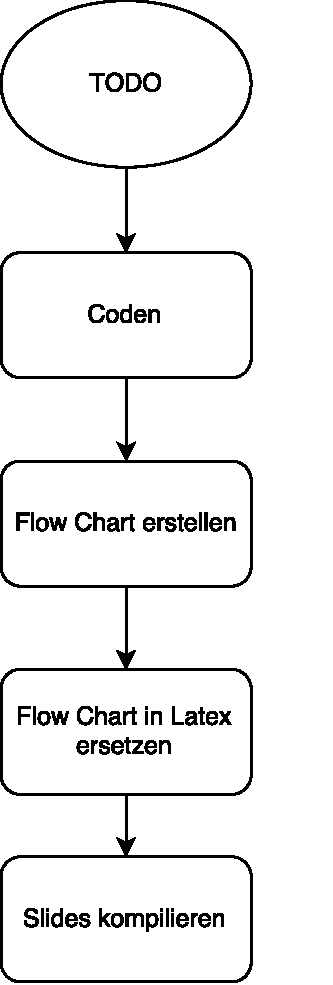
\includegraphics[scale=0.3]{FlowChartTodo.pdf}
\end{frame}

\subsection{Verwendete Funktionen}
%\begin{frame}[fragile]{Funktion loaded\_random\_choice(..)}
  \begin{itemize}
    \item Diese Funktion verlangt eine WSKL Liste als Eingabeparameter
    \item Gibt einen Index zurück, welcher 0 bis $\left\vert{probality\_list}\right\vert-1$ sein kann.
    \item Diese Indizes haben eine gewichtete WSKL, welche jeweils an der Position in der Eingabeliste steht
    \item Beispiel probility\_list := [ 0.9, 0.1 ]  $\Rightarrow$ mit p=90\% wird 0 zurückgegeben, p=10\% für 1
  \end{itemize}
  \begin{lstlisting}[language=python]
def loaded_random_choice(probability_list):
    n = len(probability_list)
    random_number = random.random()
    cum_p = 0
    for i in range(n):
        cum_p += probability_list[i]
        if cum_p > random_number:
            return i
    return None
\end{lstlisting}
\logopythonbottom
\end{frame}	

\section{Ergebnisse}
\begin{frame}[fragile]{Simulationsergebnis Var 1, Bsp 1}
    	\begin{figure}[h!]
    	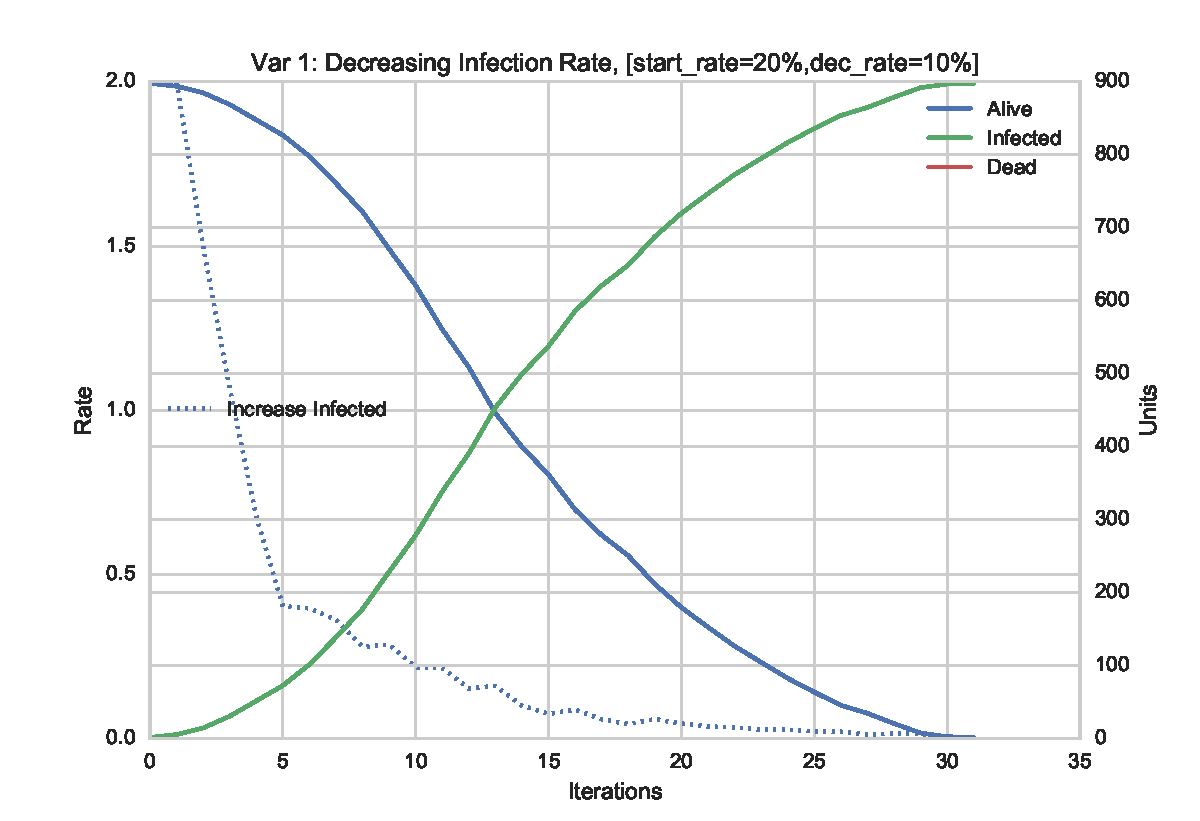
\includegraphics[scale=0.5]{BSP27_Plot_1.pdf}
		\end{figure}
\end{frame}

\begin{frame}[fragile]{Simulationsergebnis Var 1, Bsp 2}
    	\begin{figure}[h!]
    	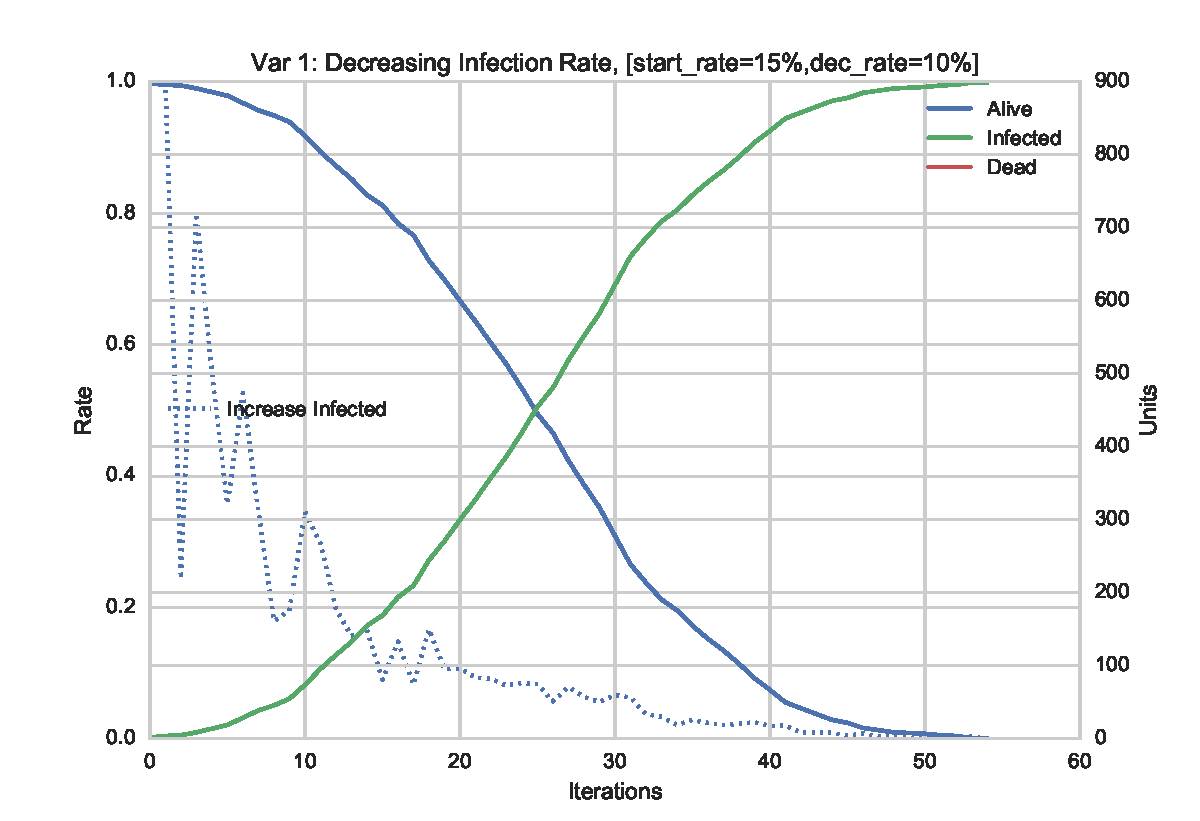
\includegraphics[scale=0.5]{BSP27_Plot_2.pdf}
		\end{figure}
\end{frame}

\begin{frame}[fragile]{Simulationsergebnis Var 2, Bsp 1}
    	\begin{figure}[h!]
    	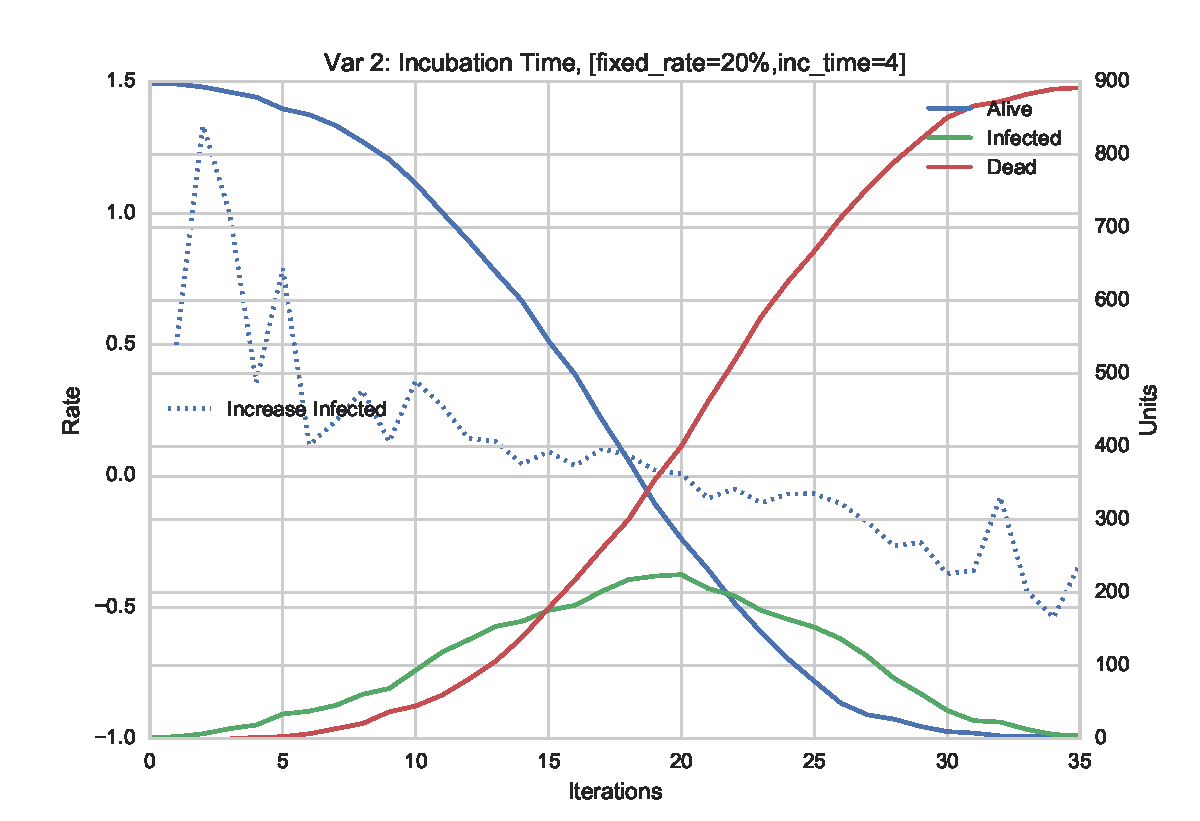
\includegraphics[scale=0.5]{BSP27_Plot_3.pdf}
		\end{figure}
\end{frame}

\begin{frame}[fragile]{Simulationsergebnis Var 2, Bsp 2}
    	\begin{figure}[h!]
    	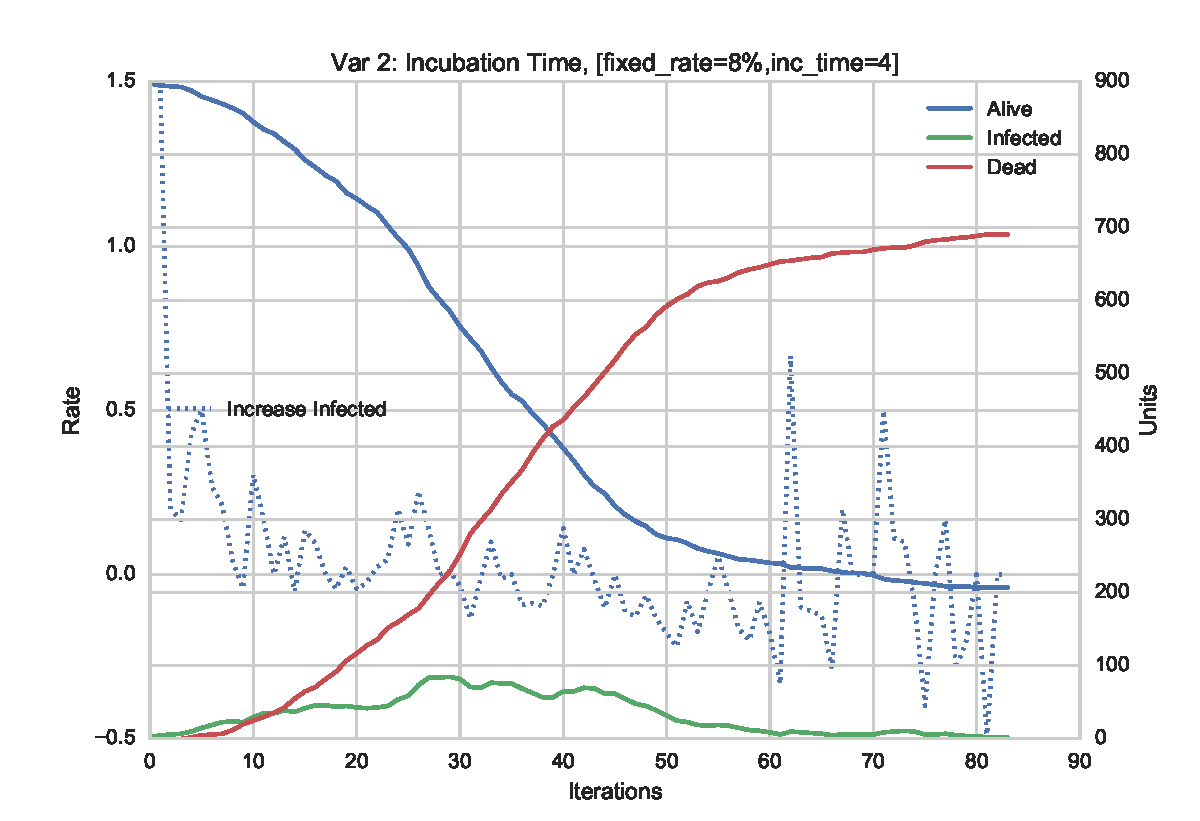
\includegraphics[scale=0.5]{BSP27_Plot_4.pdf}
		\end{figure}
\end{frame}

\end{document}
